\documentclass[9pt,twocolumn,twoside]{../../styles/osajnl}
\usepackage{fancyvrb}
\usepackage{listings}
\usepackage{hyperref}

\journal{i524} 

\title{Deploying a spam message detection application using R over Docker and Kubernetes}

\author[1,*]{Sagar Vora}
\author[1]{Rahul Singh}

\affil[1]{School of Informatics and Computing, Bloomington, IN 47408, U.S.A.}

\affil[*]{Corresponding authors: vorasagar7@gmail.com, rahul\textunderscore singh919@yahoo.com}

\dates{project-P007, \today}

\ociscodes{Docker, Ansible, Kubernetes, R, Pandas, Spam, <add spam detection algorithms>}

% replace this with your url in github/gitlab
\doi{\url{https://github.com/cloudmesh/sp17-i524/raw/master/project/S17-IR-P007/report/report.pdf}}

\begin{abstract}
 
In the last few decades, online spam has become one of the major
problem for the sustainability of the Internet. Due to the excessive
amount of spams, the quality of information available on the Internet
has reduce drastically. Moreover spam messages are also creating
problems among the various search engines available and the web
users. This report aims at developing an application which would
detect spam messages from actual meaningful messages using Pandas and
R. For the purpose for parallelizing the process, we would deploy the
application using Docker containers on the Kubernetes cluster using
ansible scripts which would automate the deployment.
 

\end{abstract}

\setboolean{displaycopyright}{true}

\begin{document}

\maketitle

\section{Introduction}

Today, the Internet \cite{www-internet} has been adopted rapidly in
the day to day life of people. It has provided a platform for
information generation and consumption. Moreover, it is used on a
daily basis to search for information and acquire knowledge. The
online encyclopedia Wikipedia™ \cite{www-wikipedia} provides a good
example of a more socialized Internet because the content within
Wikipedia™ is collectively generated by its users, rather than
webmasters or designated editors. The ease with which content can be
generated and published has also made it easier to create spam. Spam
can be stated as any information which does not add value to a user of
the web. Messages which are inappropriate, unsolicited, repeated and
irrelevant can be all classified as spam.

\noindent
So in this report, we are provinding an application that would
identify valid messages and spam messages from a given dataset. For
spam detection, we are using various techniques like Bayesian, <text
here> ...... Moreover, deploying our application using Docker
\cite{www-docker-about} containers on the Kubernetes
\cite{www-kubernetes} cluster will give a distributed approach.This
would also speed up the process of identifying the spam messages. We
have also deployed it on different cloud environments like Chameleon,
JetStream, FutureSystem and have performed benchmark analysis of the
application. This would let us the time taken by the algorithm on
these cloud solutions.

\section{Software Stack}

\begin{figure}[ht]
\begin{center}
 \begin{tabular}{|c | c|} 
 \hline
Name of the Technology & Purpose in the Project \\ [0.5ex] 
 \hline\hline
    
R & data analytics \\
\hline

Docker & container for the application \\
\hline

Kubernetes & cluster creation and management \\[1ex]
\hline

Cloudmesh Client & An client application used to ssh in various cloud
environments \\[1ex]

\hline
Ansible & Automation language to deploy
application on the target machines \\[1ex]
\hline

\end{tabular}
\end{center}
  \caption{Technologies used in the Project}
\end{figure}

\section{ELEMENTS OF THE PROJECT}

\subsection{Ansible}
No one likes repetitive tasks, so with Ansible \cite{www-ansible}, IT
admins can begin automating away the drudgery from their daily routine
tasks. Ansible is a simple automation language that can perfectly
describe an IT application infrastructure. Ansible is an open source
automation engine which can be used to automate cloud provisioning,
configuration management, and application deployment. It can also
perform more advanced IT tasks such as continuous deployment or
rolling out updates with zero downtime.

A major difference in Ansible and many other tools in the
space is its architecture.

\subsubsection{Architecture}
Ansible is an agentless tool,it doesn't requires any software to be
installed on the remote machines to make them manageable. By default
is manages remote machines over SSH or WinRM, which are natively
present on those platforms \cite{www-ansible-architecture}.

Like the other configuration management software, Ansible
distinguishes between two types of servers: one being the controlling
machines and other being the nodes. Ansible uses a single controlling
machine where the orchestration begins. Nodes are then controlled by a
controlling machine over SSH \cite{www-ssh}. The location of the nodes
are described by the inventory of the controlling machine.

Ansible modules are deployed by Ansible over SSH. These modules are
temporarily stored in the nodes and communicate with the controlling
machine through a JSON protocol over the standard output

\subsubsection{Playbooks}

Playbooks \cite{www-ansible-playbook} are Ansible’s configuration,
deployment, and orchestration language. They let us control the remote
systems with a policy which we might want them to enforce. If Ansible
modules act as tools in your workshop, then playbooks are your
instruction manuals, and your inventory of hosts are your raw
material. Playbooks can be used to manage configurations of and
deployments to remote machines. They can sequence multi-tier rollouts
involving rolling updates, and can delegate actions to other hosts,
interacting with monitoring servers and load balancers.

\subsubsection{Ansible Galaxy}

\subsection{R}
R is a language and environment for statistical computing and graphics
\cite{www-about-rproject}. Pandas does not provide a significant
statistical modeling environment as it is still a work in progress. R
provides a variety of statistical model analysis, classification,
clustering and graphical techniques to provide this
environment. Integrating Python's efficiency with R's capability
allows us to build a highly a desirable analysis model for our
application.


\subsection{Docker}

\emph{Docker} is an open-source project that automates application
deployment by packaging the application in
\emph{containers}. Containers provide application portability by
bundling together an application and its needed resources in a package
so that they can be deployed on different platforms without worrying
about resource dependencies. Application containerization is an OS
(Operating System) level emph{virtualization} for deploying and
running an application instance without launching a virtual mahine for
each application \cite{www-containerization}. A container has its own environment
variables, filesystem and libraries that is needed by the application,
thus eliminating OS or hardware dependency. Containers abstract the OS
kernel while a \emph{VM (Virtual Machine)} hypervisor abstracts an
entire device.

Docker allows application developers to package their applications
into isolated containers. Docker automates the repetitive tasks of
setting up and configuring development environments thus allowing
developers to focus only on building software. A dockerized
application can simply ship between platforms as the complexity of
software dependencies is handled by the container.  Docker
standardizes container creation and can be used to pack, ship and run
an application as a lightweight container that can run in any
environment. Docker can be integrated with other devops applications
like Puppet, Chef, Vagrant, Ansible and Kubernetes. We shall use
Docker with Ansible and Kubernetes in our project.

\subsubsection{Dockerfile and DockerImage}
To package an application and its dependencies in a single file,
docker introduces the concept of a \emph{docker image}. The docker
engine creates a docker image by parsing contents of a
\emph{dockerfile}. A dockerfile is a script composed of various
commands to build a container in a step-by-step, layer-by-layer manner
\cite{www-docker-digitalocean}. Once an image has been built it can be shared with other
users by pushing it to a public repository on \emph{DockerHub} or
\emph{GoogleCloudPlatform}. In this manner, an image once built by the
docker engine can be used across the organization by making a docker
pull request.

\subsection{Kubernetes}
Kubernetes is an open-source platform for automating deployment,
management and scaling of containerized applications across a cluster
\cite{www-wiki-kubernetes}. The more granular an application is, the more components it
consists of and thus requires management of these
components. Kubernetes helps in faster deployment of applications and
scaling them on the fly. Moreover it optimizes the use of hardware by
using the resources which are needed. Kubernetes provides container
management features like component replication, load-balancing,
service-discovery and logging across components \cite{www-kubernetes-architecture}. A Kubernetes
cluster can be deployed on either physical or virtual machines. We
shall be deploying a kubernetes cluster using \emph{kubeadm} - the
kubernetes command line tool and \emph{Minikube} which is a
lightweight Kubernetes implementation which creates a VM on the local
machine and deploys a simple cluster containing only one node. The
Minikube CLI provides basic bootstrapping operations for working with
the cluster, including start, stop, status, and delete commands.

\subsection{Kubernetes Terminologies}
Kubernetes defines the following set of primitives which provide
mechanisms for deploying and scaling applications.

\subsubsection{Pods}
A pod is the smallest unit of a kubernetes cluster and has a unique
ip-address within the cluster. A pod consists of one or more
containers that can share resources and can be controlled as a single
application \cite{www-wiki-kubernetes} \cite{www-kubernetes-digitalocean}. Thus all the involved containers in a
pod are scheduled on the same host. A pod can be thought of as a
single virtual machine in terms of resource sharing and scheduling.
Pods can be managed manually using the \emph{Kubernetes API} or can be
managed by a controller.

\subsubsection{Services}
A kubernetes service is a collection of pods that perform the same
function and are presented as a single entity. This way a service can
be emphasized as a one tier of a multi-tier application. Service act
as an interface to a group of containers so that service-consumers
need only reference the single access location. Kubernetes facilitates
service discovery by assigning a stable IP address and a namespace to
a service. This idea abstracts the change of IP addresses of pods
within a service that result due to pod failure or pod rescheduling.

\subsubsection{Replication Controllers}
A replication controller is a framework for horizontal scaling of
pods. Semantics of a pod are defined in a <pod\textunderscore name>.yaml file which
also defines the replication details that need to be done. The
replication controller performs replication by scaling a number of
pods across a cluster based on the pod definition file \cite{www-wiki-kubernetes}. The
replication controller has to make sure that a certain number of
copies of a pod are always up and running. Thus, in event of a pod
failure it replaces the failed pod with a new replica.

\subsubsection{Labels and Selectors}
Kubernetes allows users or internal components to assign a key-value
pair tag to any API object in the system. An object can have one or
more labels associated with it, but each with a unique key. eg:
appversion = 1.0, development\textunderscore stage = 4.  Label selectors are queries
against labels that return matching objects \cite{www-kubernetes-digitalocean}. This way each
object in the system can be referenced with a single label or a
combination of multiple labels for fine grained control.

\subsection{Kubernetes architecture}
Kubernetes exhibits the master-slave architecture. The components can
be split into those that manage an individual node(slave) and those
that manage the master or control plane.

\begin{figure}[htbp]
\centering
\fbox{\includegraphics[width=60mm,height=60mm]{images/kubernetesArchitecture.JPG}}
\caption{Kubernetes architecure \cite{www-kubernetes-architecture}}
\label{fig:Kubernetes Minimum Architecture}
\end{figure}


\textbf{Kubernetes Master Node/Control plane}
\newline
The Kubernetes master node is responsible for managing the kubernetes
cluster and orchestrating the worker nodes, where the actual pods are
scheduled. The master node can work as a single node cluster where it
can schedule pods to work on the master node itself by tainting the
schedule policy rule on the node. The master node also referred as
the control plane consists of several components:

\subsubsection{API Server}
The API server is the most fundamental component of the Kubernetes
master and serves as the entry point for all the REST commands used to
control the cluster. The API server serves up the Kubernetes API using
JSON over HTTP, providing both internal and external interface to the
cluster \cite{www-kubernetes-digitalocean}
\cite{www-apiserver-kmblog}. It validates the REST requests, executes
them and updates the status of the objects in the \emph{etcd} storage.

\subsubsection{etcd storage}
\emph{etcd} is a simple, distributed and consistent key-value store
that stores configuration data of the cluster and represents the state
of the cluster at any point of time
\cite{www-wiki-kubernetes}. Kubernetes uses etcd for service discovery
and provides a simple HTTP/JSON API as an interface for setting or
retrieving values from the store. Other components watch the state of
the etcd store to bring themselves up to the desired state. Data being
stored in the etcd store are deployed services, pods, replication
information etc.

\subsubsection{Scheduler}
The scheduler component is responsible for the deployment of pods and
services on the cluster nodes. The scheduler has the information about
the availability of resources on a node and schedules unscheduled pods
on the nodes accordingly. Along with scheduling, the scheduler also
tracks resource utilization of each node and ensures that workload
scheduled is not in excess to the resources available \cite{www-wiki-kubernetes}.

\subsubsection{Controller-manager}
The controller manager is the process embedding the different types of
controllers like the Replication Controller or the DaemonSet
Controller on a kubernetes master. The controllers query the API
Server to manipulate the resources like pods,services etc. which they
manage.

\subsection{Worker Node}
The worker node also called as minion node is where the containers are
actually deployed. The worker contains all the necessary services
needed to manage the networking between containers, communicate with
the master node and assign resources to the scheduled containers
\cite{www-kubernetes-architecture}.  Every worker node must run the container runtime i.e docker
and other components stated below to ensure proper communication with
the master.

\subsubsection{Docker}
Docker runs on each of the worker nodes. It is responsible for
downloading the docker images and running the configured pods by
starting the container.

\subsubsection{Kubelet}
\emph{Kubelet} gets the pod definition from the api-server and is
responsible for maintaining the pod in the desired state. Kubelet is
the worker service that monitors the health of each pod and
communicates the status of each node via a heartbeat message to the
master.  If the pod is not in the desired state, it is redeployed to
the same node \cite{www-wiki-kubernetes}. Kubelet is also responsible for communicating
with the etcd storage to get information about the services and update
the storage about newly created ones.

\subsubsection{Kube-Proxy}
\emph{Kube-proxy} acts as a network proxy and a load balancer. It is
responsible for networking of TCP and UDP packets to the appropriate
container based on the IP address of each packet
\cite{www-wiki-kubernetes} \cite{www-kubernetes-architecture}.

\subsubsection{Kubectl}
\emph{kubectl} is a command line tool that communicated with the API
server to fetch important information about the nodes, pods, services
and events in the cluster.


\section{Design}
\subsection{Building the Classification model}

\subsubsection{CrossValidation for the training data}

To address the problem of incoming spam messages, a model shall be
developed using the Bayesian Classification technique to correctly
classify each incoming email/text message as a spam or a legitimate
one. The model aims at developing a message filter that shall
correctly classify messages based on word probabilities that are
extracted from the training dataset.The training dataset to build the
model consists of 5574 message records. Dataset taken from
\cite{www-sms-spam-dataset}. The training process shall use the
cross-validation feature provided by R to build the classification
model and use Bayes theorem of conditional probability to predict the
class of each incoming message.

To develop an efficient training model, we shall partition the data
into 2 subsets - training data and classification data. We shall
choose one of the subsets for training and other for testing. In the
next iteration the roles of the subsets shall be reversed, i.e the
training data becomes the classification one and vice versa. This
operation shall be carried out until each individual record is used
both as a classification and training record. We shall use the cross
validation feature provided by R for this subsampling. This
subsampling technique handles the underfitting problem and guarantees
an effective classification model.


\subsubsection{Training process}
Content of each of the spam marked messages shall be processed through
Naive Bayes Classifier.  The classifier shall maintain a bag of words
along with the count of each word occuring in the spam messages. This
word count shall be used to calculate and store the word probability
in a table that shall be cross-referenced to determine the class of
the record on classification
data \cite{paper-classification-of-email}.

A selected few words have more probability of occuring in a spam
messages than in the legitimate ones. Eg: The word "Lottery" shall be
encountered more often in a spam message.  The classifier shall
correlate the bag of words with spam and non-spam messages and then
use Bayes Theorem to calculate a probability score that shall indicate
whether a message is a spam or not. The results shall be verified with
the results available on the training dataset and the classifier
accuracy shall be calculated.  The classifier shall use the Bayesian
theorem over the training dataset to calculate probabilities of such
words that occur more often in spam messages and later use a summation
of scores of the occurence of these word probabilities to estimate
whether a message shall be classified as spam or not. After working on
several samples of the training dataset, the classifier shall have
learned a high probability for spam based words whereas, words in
legitimate message like family member or friends names shall have a
very low probability of occurence.

\subsection{Classifying new data}

Once the training process has been completed, the posterior
probability for all the words in the new input email is computed using
Bayes theorem. A threshold value shall be defined to classify a
message into either class. A message's spam probability is computed
over all words in its body and if the sum total of the probabilities
exceeds the predefined threshold, the filter shall mark the message as
a spam \cite{www-wiki-naivebayes}.

A higher filtering accuracy shall be achieved through filtering by
looking at the message header i.e the sender's number/name. Thereby if
a message from a particular sender is repeatedly marked as spam by the
user, the classifier need not evaluate the message body if it is from
the same sender.

\section{DEPLOYMENT}
Our application will be deployed using Ansible \cite{www-ansible}
playbook. Automated deployment should happen on two or more nodes
clouds or on multiple clusters of a single cloud. Deployment script
should install all necessary software along with the project code to
Kubernetes cluster nodes using the Docker image.

\subsection{Deployment process - Ansible}
<TODO - describe the ansible deployment and scripts>

\subsection{Dockerizing the application}
To containerize our application, we need to create a docker image for
it. To create a docker image we need to create a docker file that
describes the semantics to create the docker image. Docker version
used for this process is 1.12.6.

\subsubsection{The Dockerfile}
Docker can build images automatically by reading instructions from a
Dockerfile. A dockerfile is a series of text commands that a user can
run on a command line to build an image \cite{www-dockerfile-documentation}.
\newline
Instructions within a Dockerfile have the following format:

\begin{verbatim}
INSTRUCTION  arguments
\end{verbatim}

Docker reads the instructions from a dockerfile in the order they are
written. The very first line of a docker file must be a 'FROM' clause
which specifies the base image from which the image is being built. As
our application works with R, we need to specify the base package as
one that shall help us run our R application. \emph{DockerHub} has a
r-base package that binds the latest version of R and its libraries
together that we shall use \cite{www-rbase-docker}.  The argument
following the FROM clause is a repository/tag name that the docker
engine automatically looks up on \url{http://hub.docker.com}.

Following the FROM statement, we can specify all actions we need to
perform like specifying the work directory for building the image or
copying files into our work directory so that every resource is
available under a single folder. Lastly, our docker file ends with a
CMD statement that specifies the command that the container is
supposed to execute on successful instantiation. CMD accepts an array
of command names followed by the parameters. Since we want our image
to execute our R application we shall specify the cmd as stated in the
dockerfile snapshot below.


\begin{figure}[htbp]
\centering
\fbox{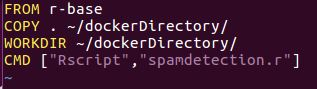
\includegraphics[width=60mm,height=15mm]{images/dockerfile.JPG}}
\caption{Dockerfile of the spam detection application}
\label{fig:Dockerfile}
\end{figure}

\subsubsection{Creating a docker image}

Once the Dockerfile is built, we can build the image using docker
build command as follows :

\begin{verbatim}
docker build -t myscript /path/to/Dockerfile
\end{verbatim}

\begin{figure}[htbp]
\centering
\fbox{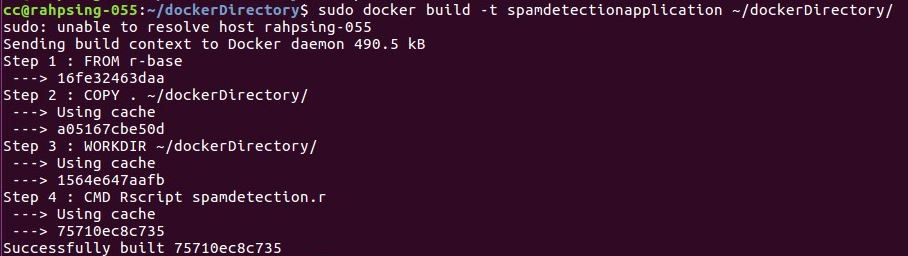
\includegraphics[width=80mm,height=30mm]{images/dockerbuild.JPG}}
\caption{Building a docker image}
\label{fig:Building the docker image}
\end{figure}



The built image is placed in our machine's local docker registry and
can be viewed with the 'docker images' command.

\begin{figure}[htbp]
\centering
\fbox{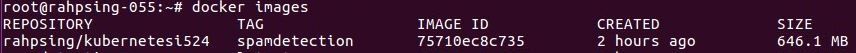
\includegraphics[width=80mm,height=10mm]{images/dockerimages.JPG}}
\caption{Output of the docker images command}
\label{fig:Docker Images on the system}
\end{figure}

\subsubsection{Running the application}

We shall run our application using the docker run command.

\begin{verbatim}
docker run spamdetection
\end{verbatim}

We can check the container id of our application along with other
important information using the 'docker ps' command.
 
\subsubsection{Sharing the docker image}

By default, the docker CLI points to docker's public registry which is
located at \url{http://hub.docker.com}. We need to create a docker
account to upload our application image so that it could be directly
referenced by kubernetes later. Once a docker account is registered,
create a public repository and give it a name. The repository shall be
accessible by the format '<username>/repositoryname'.

To tag the current docker image that we created on our system we need
to inform the docker engine to point to our registry. To do so, we
shall use login command provided by the docker CLI.

\begin{verbatim}
docker login
\end{verbatim}

The login request shall ask for a valid docker account userid and
password. Once authenticated, the docker engine shall establish a link
with the registry associated with the username.  To upload our docker
image to the repository, we need to tag the image. Docker provides the
'tag' command to do so.

\begin{verbatim}
docker tag image_name <username>/<repository_name>:<tag>
\end{verbatim}

The <tag> can be any name given by the user to uniquely identify the
image. Once tagged, we need to push the image to the repository using
the command line 'docker push' command.

\begin{verbatim}
  docker push rahpsing/kubernetesi524:spamdetection
\end{verbatim}


As the image is now publicly available on the repository, we can do a
simple 'docker pull' from any machine to deploy the container with no
dependencies. This is possible as the image wraps together the
application code file, the data file and dependent r-base package from
the latest version of R available on dockerhub's library.


\subsection{Deployment via Minikube}
<TODO - install minikube, deploy image on minikube created kubernetes cluster>

\subsection{Deployment via kubeadm}
<TODO - install kubectl,kubeadm, deploy the application and check status>

\section{Issues tackled with Kubernetes setup and deployment}
<TODO: describe IMAGEPULLBACKOFF, CRASHLOOPBACKOFF,
Weave-net daemon set, master taint issue, issues with ubuntu 14.04>

\section{Discussion}
TBD

\section{Conclusion}

TBD

\section{Acknowledgement}

We acknowledge our professor Gregor von Laszewski and all associate
instructors for helping us and guiding us throughout this project.

\section{Appendices}
TBD

% Bibliography

\bibliography{references} 

\end{document}
